% !TeX root = ../main.tex
% Add the above to each chapter to make compiling the PDF easier in some editors.

\chapter{Experiments}
\section{Pilot Studies}
Prior to the \nameref{final_study} study, two pilot studies were conducted: \nameref{study_one}, and \nameref{study_two}. This was done to study certain aspects of the final study separately, and make decisions, such as what sound type (earcons or auditory icons) to choose, and at what speed to translate the buildings.

\subsection{Sound Speed and Type}
\label{study_one}
% Goal of the study

\paragraph{Methods}

% Participants

% Procedure

% Task

% Apparatus (i.e Unity, Resonance Audio, stereo headphones, Vive)

% Study Factors and Conditions: what my factors are, conditions == independent variables' values

\subsection{Spatial Judgement}
\label{study_two}
\section{Workspace Awareness in Immersive Virtual Reality}
\label{final_study}
% Goal of the study
The goal of this study was to analyze \gls{wa} that participants have of others present in the same immersive \gls{vr} environment. Participants were presented with a primary and secondary tasks. Primary task was tracing 3D models with a 3D brush, and secondary task was a \gls{wa} task - reporting changes to the environment.

\paragraph{Methods}
Aspects of \gls{wa} that were evaluated was participants’ reaction speed when provided with different types of awareness presentation (audio and/or visual cues from the environment).

% Participants
12 participants (8 men and 4 women) were recruited among friends, employees from the chair, and students from the \gls{tum}; ages ranged from 22 to 32 (mean 25.2, std. 2.5). Only one participant reported having "partially" good hearing, others reported good hearing. 3 people reported to be familiar with \gls{vr} technology, among them, one person reported being a proficient gamer and one - having partaken in driving simulator studies. Participants were a mix of gamers, non-gamers, and casual gamers. Participants were also equally distributed among people who had experience with \gls{vr}, those who had some experience, and those who had no prior experience. Two reported being online gamers, and another two - occasional online gamers. Only one person had prior experience with architecture, and had worked in the field. One participant tried 3D drawing in the system, but otherwise none of the participants had seen the system before, or took part in the trial studies.

% Procedure
Participants were given a written and verbal introduction to the experiment,
after which were asked to sign the consent form for using their data.
Next, participants went through the tutorial, where the 3D brush, laser pointer for pinpointing the buildings and auditory cues were introduced. Participants went through a small scenario resembling the actual experiment, where they were asked to trace a pillar, while catching a moving building, and keeping track of how the building sounds and where it is visually.
During the actual experiment, each participant was tested in each of the 3 test groups.
At the end of the experiment, participants were asked to fill in a self-report questionnaire.
Participants did not rest between the different conditions. 

% Task
Participants were tasked with the scenario, in which there are 2 architects (A1 and A2), who perform their separate tasks in the same urban district (\ref{fig:urbandistrict}) in \gls{vr}. A1 (participant) has 2 tasks: primary and secondary. The primary task is to trace given 3D shapes with a 3D brush (a tracked 6-\gls{dof} controller). Meanwhile, A2 (simulated ivisible user) can translate any building in the district to any other part of the district at any time. The secondary (workspace awareness) task of A1 is to keep track of changes to the environment and pinpoint them with a virtual laser pointer (another tracked 6-\gls{dof} controller).

\begin{figure}
	\centering
	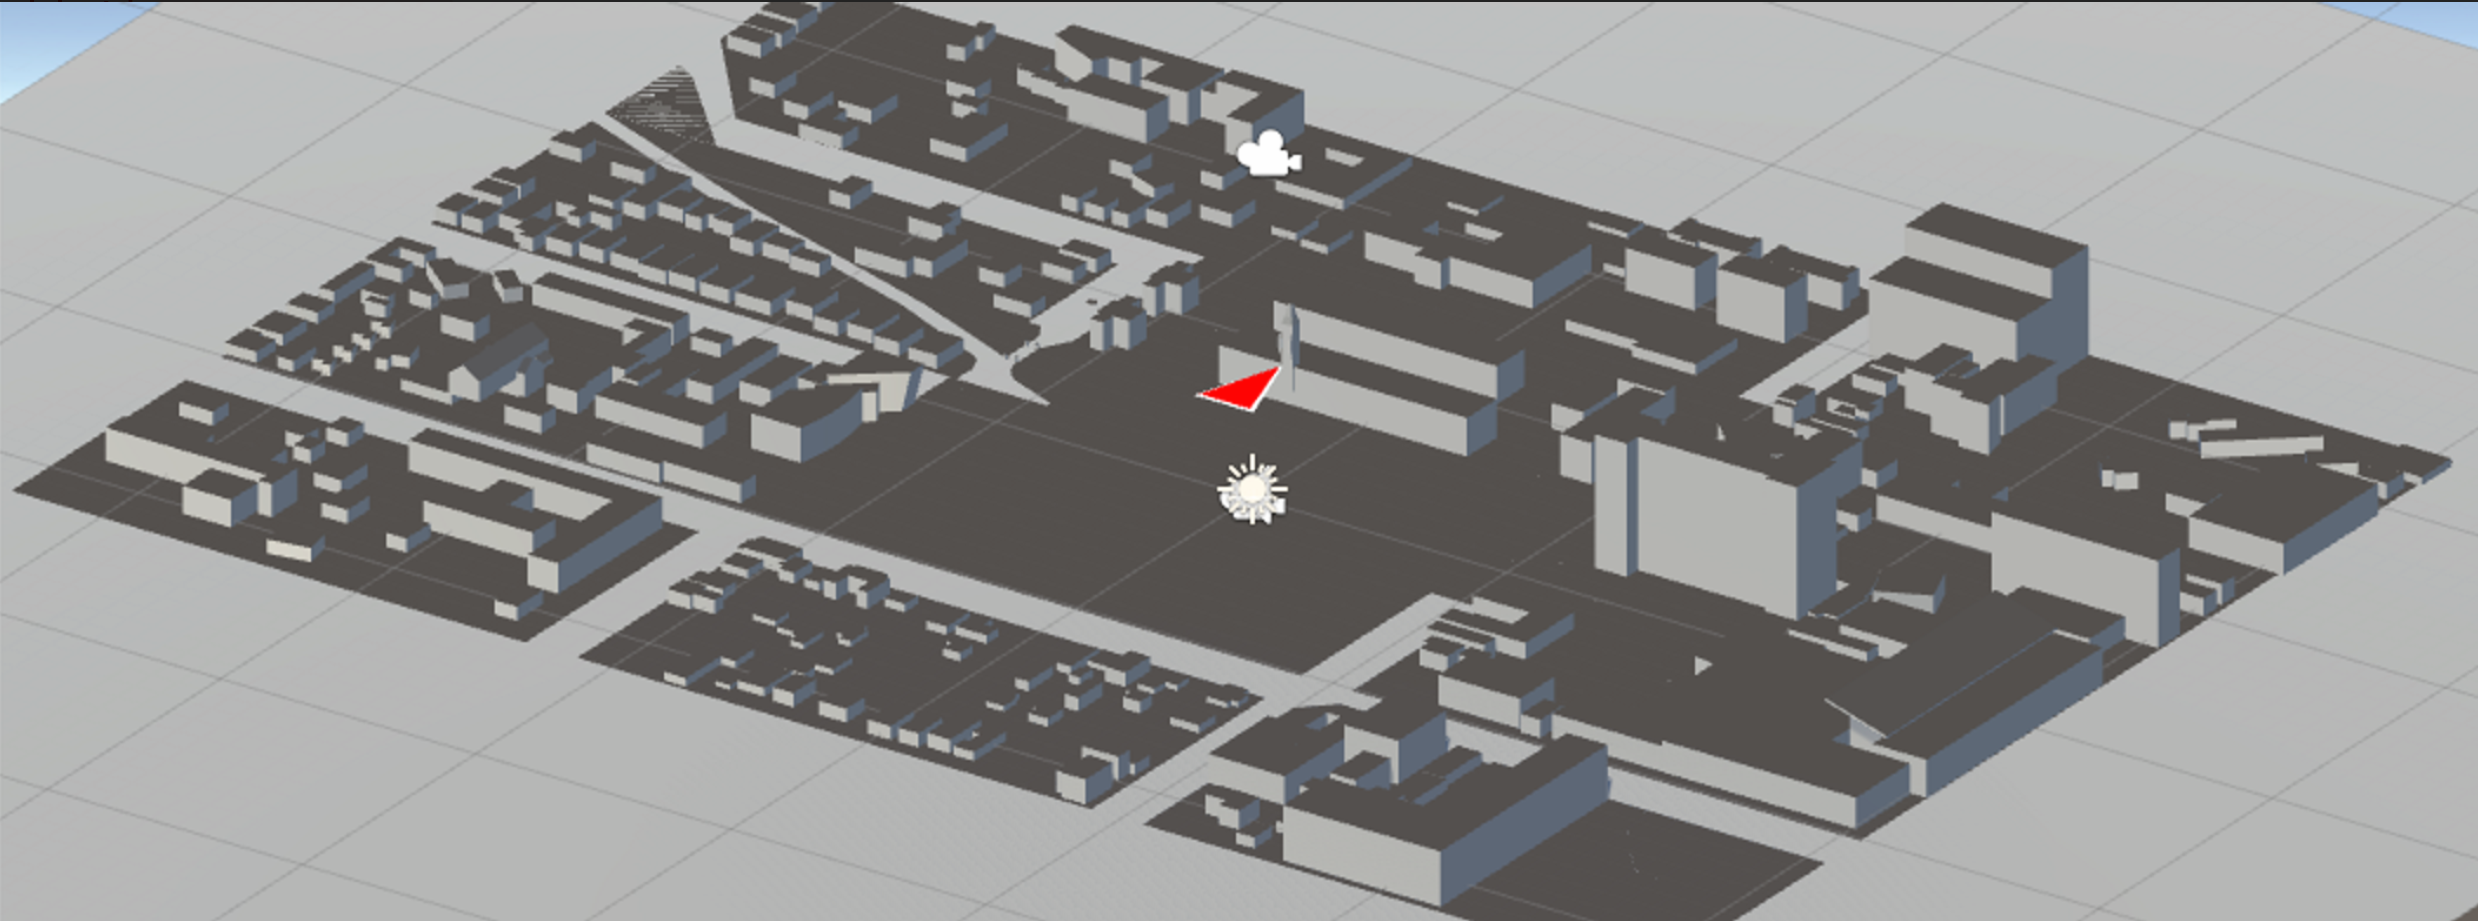
\includegraphics[width=0.7\linewidth]{figures/urban_district}
	\caption{Simulated urban district for the \gls{wa} study}
	\label{fig:urbandistrict}
\end{figure}


% Apparatus: Unity, Resonance Audio, stereo headphones, Vive
Experiment was implemented with the help of Unity3d, version  2018.1.5f1 and Resonance Audio SDK for Unity, version 1.2.1 with sound occlusion turned off. For the hardware, \gls{vr} headset and controllers from the HTC Vive were used, along with on-ear stereo headphones, and a Windows 10 PC (TODO: specs).

% Study Factors and Conditions: what my factors are, conditions == independent variables' values
\textit{Experimental Design} 
The study examined one independent variable: type of awareness presentation. 3 controlled awareness presentations  were made available to the participants: a minimap of the district (\ref{fig:minimap_controller}), auditory cues emitted by translating buildings in the scene (sound of concrete sliding on concrete), and their combination. Awareness presentations were rotated for each participant, so that each presentation was seen in the same position equal number of times. 
Each awareness presentation was tested for 10 minutes, during which exactly 8 buildings were chosen and translated randomly. There were 24 data points measured per user in each session. Data collected were the reaction speed in determining the position of a moving \gls{vb}, along with 3D drawings created by participants.

\begin{figure}[h]
	\centering
	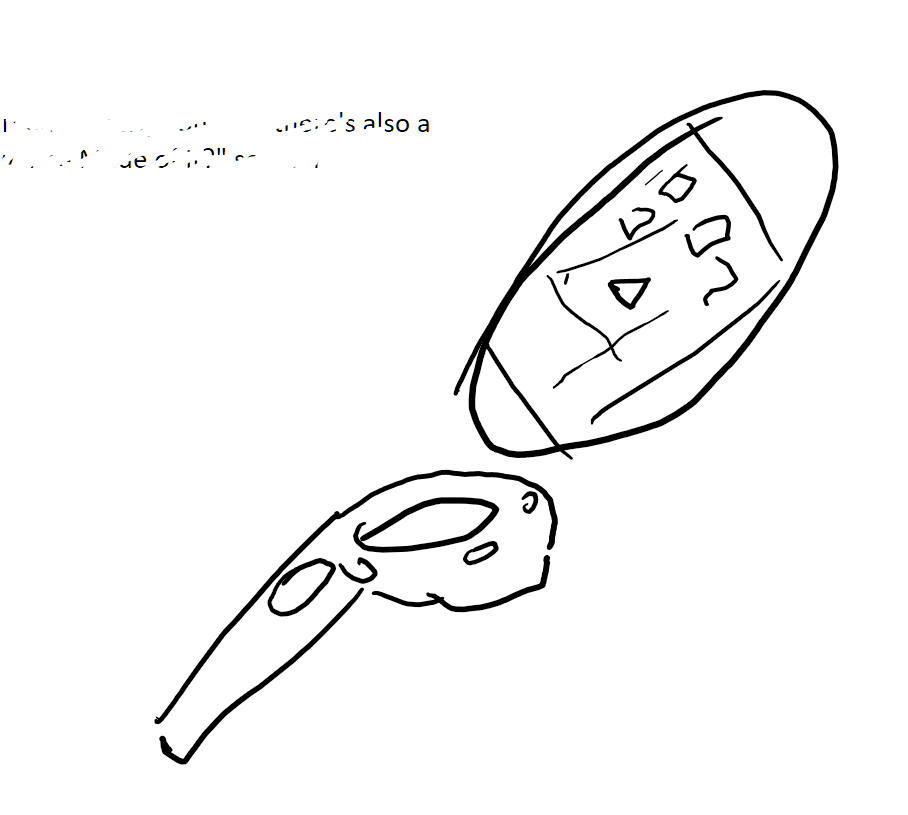
\includegraphics[width=0.7\linewidth]{figures/placeholders/minimap_controller}
	\caption{Controller with the minimap}
	\label{fig:minimap_controller}
\end{figure}


\paragraph{Gutwin vs our study}
% TODO: add a pic: Gutwin's (vertical) and our (horizontal) working (sound) plane
Since, this study extends upon \cite{gutwin_chalk_2011}, in this paragraph I provide a comparison of the two.
The main difference between - workspace is no longer a 2D plane, but an immersive 3D \gls{vr} environment. An important change here is the fact that participants are able to look around at the workspace, and notice some changes to the environment, even without the help of the minimap or auditory cues.
Second distinction is in the primary task of the participant and the simulated agent. In \cite{gutwin_chalk_2011} the participant performs the same task, as an agent: drawing with chalk. Additionally, the participant's actions emit the same sound (even though, at a lower volume) as the drawings of the agent. In this study, the primary task of the participant is - 3D drawing with voxels. This activity doesn't emit any sound. It is also different from the agent's task - translation of buildings in the urban district. Nevertheless, the tasks are still contextually related with regards to the architectural activity in urban environment.
\cite{gutwin_chalk_2011} do not specify the audio plane, in which the sound was simulated, in this experiment, the place was horizontal (TODO: ref figure). 

\begin{figure}[h]
	\centering
	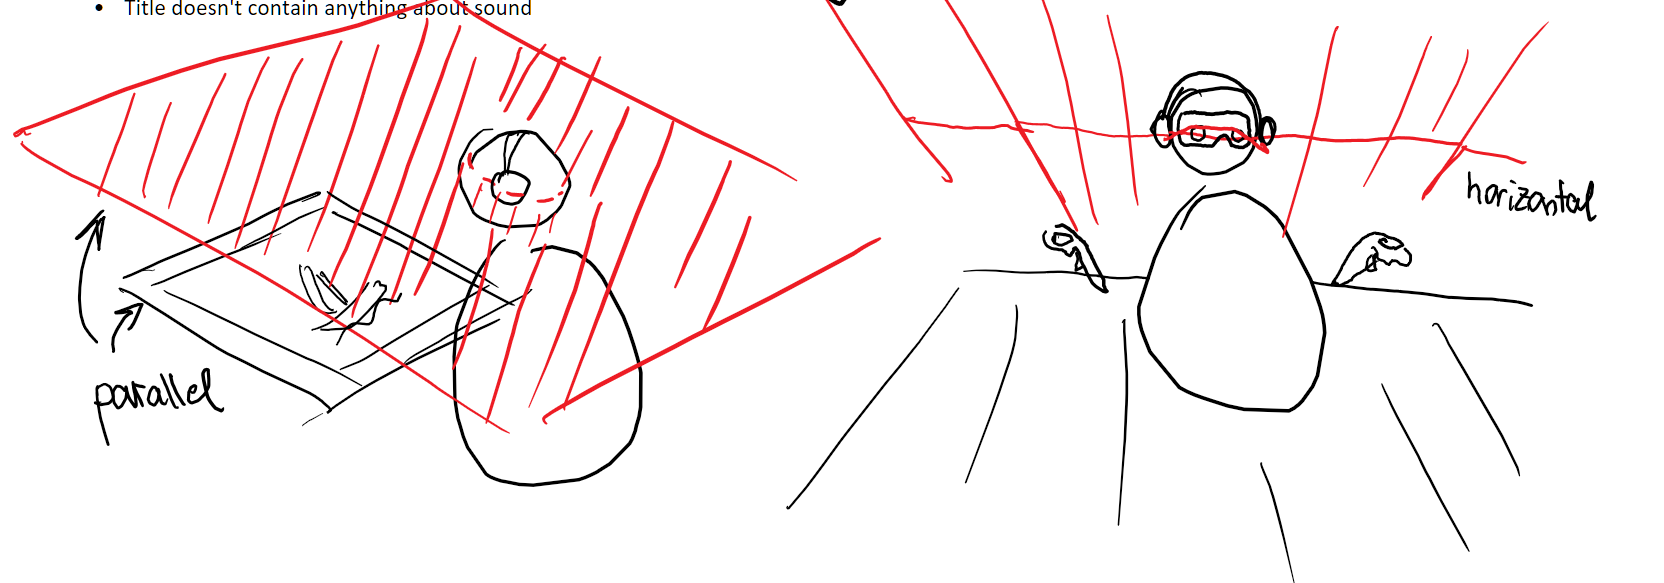
\includegraphics[width=0.7\linewidth]{figures/gutwin_vs_my_study_sound_plane}
	\caption{\cite{gutwin_chalk_2011} sound plane vs this study}
	\label{fig:gutwinvsmystudysoundplane}
\end{figure}


\begin{table}[]
  \caption{Study comparison: \cite{gutwin_chalk_2011} vs \gls{wa} in Immersive \gls{vr}}
  \label{table:study_comp}
  \begin{tabular}{|l|l|l|}
  \hline
                             & \cite{gutwin_chalk_2011}                & This study           \\ \hline
  Workspace dimensions				 & 2D									   & 3D \\ \hline
  Primary (distraction) task & The same as the primary for the simulated actor & Contextually related \\ \hline
  Working (sound) plane      & Variable             & Horizonatal          \\ \hline
  Sound type                 & Auditory icons        & Auditory icons       \\ \hline
  Object of analysis         & Workspace awareness   & Workspace Awareness  \\ \hline
  \end{tabular}
\end{table}

\paragraph{Results}

\paragraph{Study limitations}
% the fact that we only sample the level 1 SA/WA (we won't be going into sampling direction of translation guesses from the participants)
% could also try to describe it according to WA framework